% Customizable fields and text areas start with % >> below.
% Lines starting with the comment character (%) are normally removed before release outside the collaboration, but not those comments ending lines

% svn info. These are modified by svn at checkout time.
% The last version of these macros found before the maketitle will be the one on the front page,
% so only the main file is tracked.
% Do not edit by hand!
\RCS$Revision: 254481 $
\RCS$HeadURL: svn+ssh://amagnan@svn.cern.ch/reps/tdr2/papers/HIG-13-030/trunk/HIG-13-030.tex $
\RCS$Id: HIG-13-030.tex 254481 2014-08-05 10:54:09Z jbrooke $
%%%%%%%%%%%%% local definitions %%%%%%%%%%%%%%%%%%%%%
%\input{commands.tex}
% This allows for switching between one column and two column (cms@external) layouts
% The widths should  be modified for your particular figures. You'll need additional copies if you have more than one standard figure size.
\newlength\cmsFigWidth
\ifthenelse{\boolean{cms@external}}{\setlength\cmsFigWidth{0.95\columnwidth}}{\setlength\cmsFigWidth{0.8\textwidth}}
\ifthenelse{\boolean{cms@external}}{\providecommand{\cmsLeft}{top}}{\providecommand{\cmsLeft}{left}}
\ifthenelse{\boolean{cms@external}}{\providecommand{\cmsRight}{bottom}}{\providecommand{\cmsRight}{right}}
%
%%%%%%%%%%%%%% custom commands %%%%%%%%%%%%%%
\newcommand{\METnomu}{\ensuremath{\MET\mathrm{no}\mu}}
\newcommand{\mH}{\ensuremath{m_{\PH}}}
\newcommand{\BRinv}{\ensuremath{\mathcal{B}(\PH\rightarrow \mathrm{inv})}}
\newcommand{\tauh}{\ensuremath{\Pgt_\mathrm{h}}\xspace}
\newcommand{\mindphiall}{\ensuremath{\mathrm{min}\Delta\phi(\MET,\mathrm{j})}}
\newcommand{\mindphileading}{\ensuremath{\mathrm{min}\Delta\phi(\MET,\mathrm{j1/j2})}}
\newcommand{\METsig}{\ensuremath{\frac{\MET}{\sigma(\MET)}}}


%%%%%%%%%%%%%%%  Title page %%%%%%%%%%%%%%%%%%%%%%%%
\cmsNoteHeader{HIG-XX-YYY} % This is over-written in the CMS environment: useful as preprint no. for export versions
% >> Title: please make sure that the non-TeX equivalent is in PDFTitle below
\title{Search for invisible decays of Higgs bosons in the vector boson fusion production mode}

% >> Authors
%Author is always "The CMS Collaboration" for PAS and papers, so author, etc, below will be ignored in those cases
%For multiple affiliations, create an address entry for the combination
%To mark authors as primary, use the \author* form
%\address[neu]{Northeastern University}
%\address[fnal]{Fermilab}
\address[cern]{CERN}
\author[cern]{The CMS Collaboration}

% >> Date
% The date is in yyyy/mm/dd format. Today has been
% redefined to match, but if the date needs to be fixed, please write it in this fashion.
% For papers and PAS, \today is taken as the date the head file (this one) was last modified according to svn: see the RCS Id string above.
% For the final version it is best to "touch" the head file to make sure it has the latest date.
\date{\today}

% >> Abstract
% Abstract processing:
% 1. **DO NOT use \include or \input** to include the abstract: our abstract extractor will not search through other files than this one.
% 2. **DO NOT use %**                  to comment out sections of the abstract: the extractor will still grab those lines (and they won't be comments any longer!).
% 3. For PASs: **DO NOT use tex macros**         in the abstract: CDS MathJax processor used on the abstract doesn't understand them _and_ will only look within $$. The abstracts for papers are hand formatted so macros are okay.
\abstract{
A search for invisible decays of Higgs bosons in
the vector boson fusion (VBF) production mode is carried out using data
recorded in 2012 at a centre-of-mass energy of 8\,TeV by the CMS
detector corresponding to an integrated luminosity of 19.2 inverse femtobarns. Limits are set on the
production cross section times invisible branching fraction, as a
function of the Higgs boson mass. Assuming standard model Higgs boson
cross sections and acceptances, the observed (expected) upper limit on
the invisible branching fraction at $m_\PH=125$\GeV is found to be
0.XX\,(0.38) at 95\% confidence level.}%!!ADD OBSERVED AFTER WE UNBLIND

% >> PDF Metadata
% Do not comment out the following hypersetup lines (metadata). They will disappear in NODRAFT mode and are needed by CDS.
% Also: make sure that the values of the metadata items are sensible and are in plain text:
% (1) no TeX! -- for \sqrt{s} use sqrt(s) -- this will show with extra quote marks in the draft version but is okay).
% (2) no %.
% (3) No curly braces {}.
\hypersetup{%
pdfauthor={CMS Collaboration},%
pdftitle={Search for invisible decays of Higgs bosons in the vector boson fusion production mode},%
pdfsubject={CMS},%
pdfkeywords={CMS, physics, Higgs}}

\maketitle %maketitle comes after all the front information has been supplied
% >> Text
%%%%%%%%%%%%%%%%%%%%%%%%%%%%%%%%  Begin text %%%%%%%%%%%%%%%%%%%%%%%%%%%%%
%% **DO NOT REMOVE THE BIBLIOGRAPHY** which is located before the appendix.
%% You can take the text between here and the bibiliography as an example which you should replace with the actual text of your document.
%% If you include other TeX files, be sure to use "\input{filename}" rather than "\input filename".
%% The latter works for you, but our parser looks for the braces and will break when uploading the document.
%%%%%%%%%%%%%%%


%\tracinginput{introduction}
The search for invisible decays of Higgs bosons has been extensively
studied in the past~\cite{Searches:2001ab,Abdallah:2003ry,Abbiendi:2006gd},
and at the LHC with the full 7 and 8 TeV datasets, by both the
ATLAS~\cite{Aad:2014iia,Aad:2013oja} and CMS~\cite{Chatrchyan:2014tja} 
collaborations. Assuming standard model (SM) Higgs boson cross sections and
acceptances, the ATLAS collaboration places an upper limit on the
Higgs boson invisible branching fraction, \BRinv, of 0.75 at 95\% CL for
$\mH=125.5$\GeV, using the associated ZH production
mode~\cite{Aad:2014iia,Aad:2013oja}. By combining both vector boson
fusion (VBF) and associated ZH production modes, the CMS collaboration
is able to set an observed (expected) upper limit on \BRinv at $m_\PH=125$\GeV of
0.58\,(0.44) at 95\% confidence level. An extensive introduction to
the motivations for such a search and an overview of the theoretical
models proposing invisible decay channels of either SM
like or heavier Higgs bosons can be found in
Ref.~\cite{Chatrchyan:2014tja}.

In the analysis presented in this letter, the sensitivity of the CMS VBF 
analysis is improved significantly through the use of a new set of signal selection criteria.
The use of these criteria is made possible by the use of a trigger from the ``parked'' data, detailed below, 
which has looser thresholds than the trigger used for the previous analysis. The total integrated luminosity re-analysed is
$19.2 \pm 0.5$ fb$^{-1}$~\cite{CMS-PAS-LUM-13-001}.

% overview
The central feature of the CMS apparatus is a superconducting solenoid
of 6\unit{m} internal diameter, providing a magnetic field of
3.8\unit{T}. Within the volume of the superconducting solenoid are a
silicon pixel and strip tracker, a lead tungstate crystal
electromagnetic calorimeter (ECAL), and a brass-scintillator hadron
calorimeter, each composed of barrel and endcap detectors. Muons
are measured with detection planes made using three technologies:
drift tubes, cathode strip chambers, and resistive-plate chambers,
embedded in the steel flux-return yoke outside the solenoid. Extensive
forward calorimetry complements the coverage provided by the barrel
and endcap detectors. Data are selected online using a two-level
trigger system. The first level (L1T), consisting of custom made
hardware processors, selects events in less than 1\mus, while the
high-level trigger (HLT) processor farm further decreases the event
rate from around 100\unit{kHz} to a few hundred Hz before data
storage. A more detailed description of the CMS apparatus, together
with a definition of the coordinate system used and the relevant
kinematic variables, can be found in Ref.~\cite{Chatrchyan:2008aa}.

In 2012, in order to make full use of the maximum storage rate available, 
two parallel data-taking streams were put in place. The first was the standard ``prompt'' data stream, 
which was reconstructed immediately. The second was the ``parked'' data stream, which 
was taken using looser versions of some of the ``prompt'' stream triggers, and
was reconstructed later on in 2013 during the long shutdown of the LHC. 

%not mandatory anymore
%The CMS experiment uses a right-handed coordinate system, with the
%origin at the nominal interaction point, the $x$ axis pointing to the
%center of the LHC, the $y$ axis pointing up (perpendicular to the LHC
%plane), and the $z$ axis along the counterclockwise-beam
%direction. The polar angle $\theta$ is measured from the positive $z$
%axis and the azimuthal angle $\phi$ is measured in the $x$-$y$ plane.
%The pseudorapidity, $\eta$, is defined as $- \ln [\tan(\theta/2)]$. 

The analysis presented here uses the same event cleaning,
object definitions and Monte Carlo (MC) samples as described in
Ref~\cite{Chatrchyan:2014tja}.

 The VBF signal is simulated using the \POWHEG 2.0 event
generator~\cite{Nason:2004rx,Frixione:2007vw,Alioli:2009je,Hamilton:2009za,Nason:2009ai,Alioli:2010xd,Re:2010bp}. The
VBF production cross sections are taken from
Refs.~\cite{Dittmaier:2011ti,Dittmaier:2012vm}. The main background
processes, namely W, Z, and $\ttbar$ produced in association with
jets, are simulated using \MADGRAPH 5.1.1~\cite{Alwall:2011uj}
interfaced with \PYTHIA 6.4.26~\cite{Sjostrand:2006za}. The QCD
multijet background is simulated with \PYTHIA
6.4.26~\cite{Sjostrand:2006za}. Detector effects are then simulated
using the \GEANTfour package~\cite{Agostinelli:2002hh}. All MC samples
are reweighted event-by-event to reproduce the distribution of minimum
bias interactions (pileup) observed in data. 

%Additional weights are applied to simulated events to
%ensure trigger efficiency, lepton identification efficiency, and
%b-tagging efficiency match measurements from data.\par}

Electrons, muons, jets and transverse missing energy are reconstructed
with a particle-flow
algorithm~\cite{CMS-PAS-PFT-09-001,CMS-PAS-PFT-10-001}. Pileup
mitigation techniques are in place to correct the objects, as
described in detail in Ref~\cite{Chatrchyan:2014tja}.

Electrons (muons) are selected in the pseudorapidity range
$\abs{\eta}< 2.4 (2.1)$ and with p$_T> 10$\,GeV. For electrons, the
$1.44 < \abs{\eta}< 1.57$ transition region between the ECAL barrel
and endcap is excluded. Different isolation and identification
criteria are used depending on whether the lepton is explicitly
required, as in control regions where tight requirements and p$_T> 20$\,GeV conditions are enforced,
or vetoed, as in the signal region where looser conditions are required. A loose
isolation requirement is still applied for veto leptons, implying that
leptons in jets will a priori not be removed. Hadronic taus are
identified using the ``hadron-plus-strips'' algorithm \cite{Chatrchyan:2012zz}
which reconstructs the main hadronic tau decay modes using charged hadrons and photons, and leads to an expected
efficiency of 55\% for a fake rate less than 3\%, for taus with
p$_{T}>20$\,GeV and $|\eta|<2.3$. MC samples are reweighted
event-by-event to match the lepton reconstruction, identification and
isolation efficiencies measured in data.

Jets are clustered using the anti-\kt clustering
algorithm~\cite{Cacciari:2008gp}, with a distance parameter of 0.5, as
implemented in the \textsc{fastjet}
package~\cite{Cacciari:fastjet1,Cacciari:fastjet2}. Jets are selected
in the pseudorapidity range $\abs{\eta}< 4.7$ and with
p$_T>30$\,GeV. Jet energy corrections are
applied~\cite{Chatrchyan:2011ds}, as well as identification criteria
to remove contributions from calorimeter noise or from pileup
interactions. Jets with a veto electron or a loose muon within $\Delta
R < 0.5$ are filtered out.

Once all particle-flow objects are identified, the negative vectorial
sum of their transverse momenta is used to define the missing
transverse energy \MET and azimuthal angle $\phi_{\MET}$. A second
quantity $\METnomu$ is defined by ignoring any identified tight muon:
$\METnomu = \MET+\sum{\vec{p}_T^{\mathrm{tight}\,\mu}}$. The
associated azimuthal angle is referred to as $\phi_{\METnomu}$. Jet
energy corrections (including effects from pileup) are propagated to
the \MET and $\METnomu$ objects.

The same analysis strategy as in Ref.~\cite{Chatrchyan:2014tja} is
used. The pair of jets from VBF production have the distinct topology of
being well separated in $\eta$, in opposite forward/backward halves of the
detector, and having a high dijet invariant mass, M$_{jj}$. Final states with
 two jets with this VBF topology and large missing transverse energy are therefore selected.

The triggers available during the 2012 varied across different data-taking periods. For each period the 
unprescaled VBF-specific trigger with the loosest selection criteria is used, this leads to three different
triggers being used in total. All three have the same L1T selection, requiring L1T \MET$>40$\,GeV
(this is calorimeter-based only, so equivalent to \METnomu). The first trigger
is the same as the prompt trigger used in
Ref.~\cite{Chatrchyan:2008aa}, and selects, among all possible jet
pairs to minimise the impact of pileup, at least one pair of PF jets
with p$_T>40$\,GeV, $\METnomu>65$\,GeV, M$_{jj}>800$\,GeV and dijet pseudorapidity difference
$\Delta\eta_{jj}>3.5$. The first (second) parked trigger selects a pair of
calorimeter jets with p$_T>35 (30)$\,GeV,
M$_{jj}>700$\,GeV and $\Delta\eta_{jj}>3.5$. To take into account the
correlations between the different variables, the efficiency of each
trigger is measured as a function of \METnomu in bins of M$_{jj}$ and
p$_T^{j2}$, using events recorded by a single-muon trigger. All MC samples are then weighted event-by-event
 by the luminosity-weighted average of the three measured efficiencies.

After applying the triggers, the data sample is dominated by QCD
multijet events. Multijet events have two very distinct origins: (1)
events with fake \MET, where the \MET comes from mismeasured jets in the
events; and (2) events with genuine \MET, where the \MET comes from the decay of
hadrons involving neutrinos, in particular heavy-flavour decays. The
fake \MET contribution can be reduced by requiring the \MET
significance \METsig, defined as the ratio of the vectorial over
scalar sums of the transverse energy of the reconstructed PF
candidates, to be large. Both components can be
reduced by isolating the \MET, by requiring that the minimum azimuthal angle separation
between any reconstructed jet with p$_T>30$ GeV and the \MET, \mindphiall, be large.

The trigger requirements together with reducing the QCD multijet
contribution to negligible levels drive the choice of the following
selection:
\begin{equation}
  \label{eq:sel}
  \begin{aligned}
    &\eta_{j1} \cdot \eta_{j2}<0,\, \eta_{j1,2}<4.7,\\
    &\text{jet\,1}\, p_{T}>50 \,\text{GeV},\, \text{jet\,2}\, p_{T}>40\,\text{GeV},\\
    &\Delta\eta_{jj}>3.6, \,\text{GeV},\, M_{jj}>1000 \,\text{GeV}, \\ 
    &\METnomu>90\,\text{GeV},\\
    & \mindphiall > 2.0,\,\METsig>4.
  \end{aligned}
\end{equation}

At this stage in the selection, the background processes leading to a
similar final state are, by order of decreasing importance: the
associated production of W and Z with jets, QCD multijet production,
all top channels (\ttbar, single top and tW channels), dibosons, and
Drell--Yan$(\ell\ell)\text{+jets}$. The selection is further optimised
by tightening the requirements listed above to find the best 95\% C.L. expected limit on \BRinv for a \mH=125 GeV Higgs boson.
 The optimal additional selection is found to be $\mindphiall > 2.3$,
p$_{T}^{j2}>45$\,GeV and M$_{jj}>1200$\,GeV, and these requirements along with those above are used to define the signal region.

Except for the very minor dibosons and DY contributions which are
directly taken from MC, all other backgrounds are normalised to the
data using independent control regions. In the case of the W, Z and top with jets processes, where there are enough 
events the control regions are the same as the signal region
except that the lepton veto is replaced by a requirement for either exactly one lepton (electron, muon or
hadronic tau), exactly two muons, or exactly one electron and one
muon, in order to enrich the sample in W, Z or top events
respectively. In the top control region, because there are not enough events and because the QCD multijet background is
negligible, the requirement on \mindphiall is dropped. In the
W$\rightarrow\tau_{\mathrm{h}}\nu$ control region, the criteria on \mindphiall is loosened to 1, and an additional requirement that the
transverse mass of the W be greater than 20 GeV is used to reject the small remaining QCD
contribution. By studying the W$\rightarrow\mu\nu$ region (which has enough events to observe the full range of the \mindphiall distribution), 
a 20\% systematic uncertainty is added to the W$\rightarrow\tau_{\mathrm{h}\nu}$ background estimate cover the small
discrepancy in shape of the \mindphiall variable observed between data
and MC. Figure~\ref{fig:vbfCR} shows the data-MC agreement that is
obtained in the $\mindphiall$ variable in each of the control regions.

\begin{figure*}[hbtp]
\begin{center} 
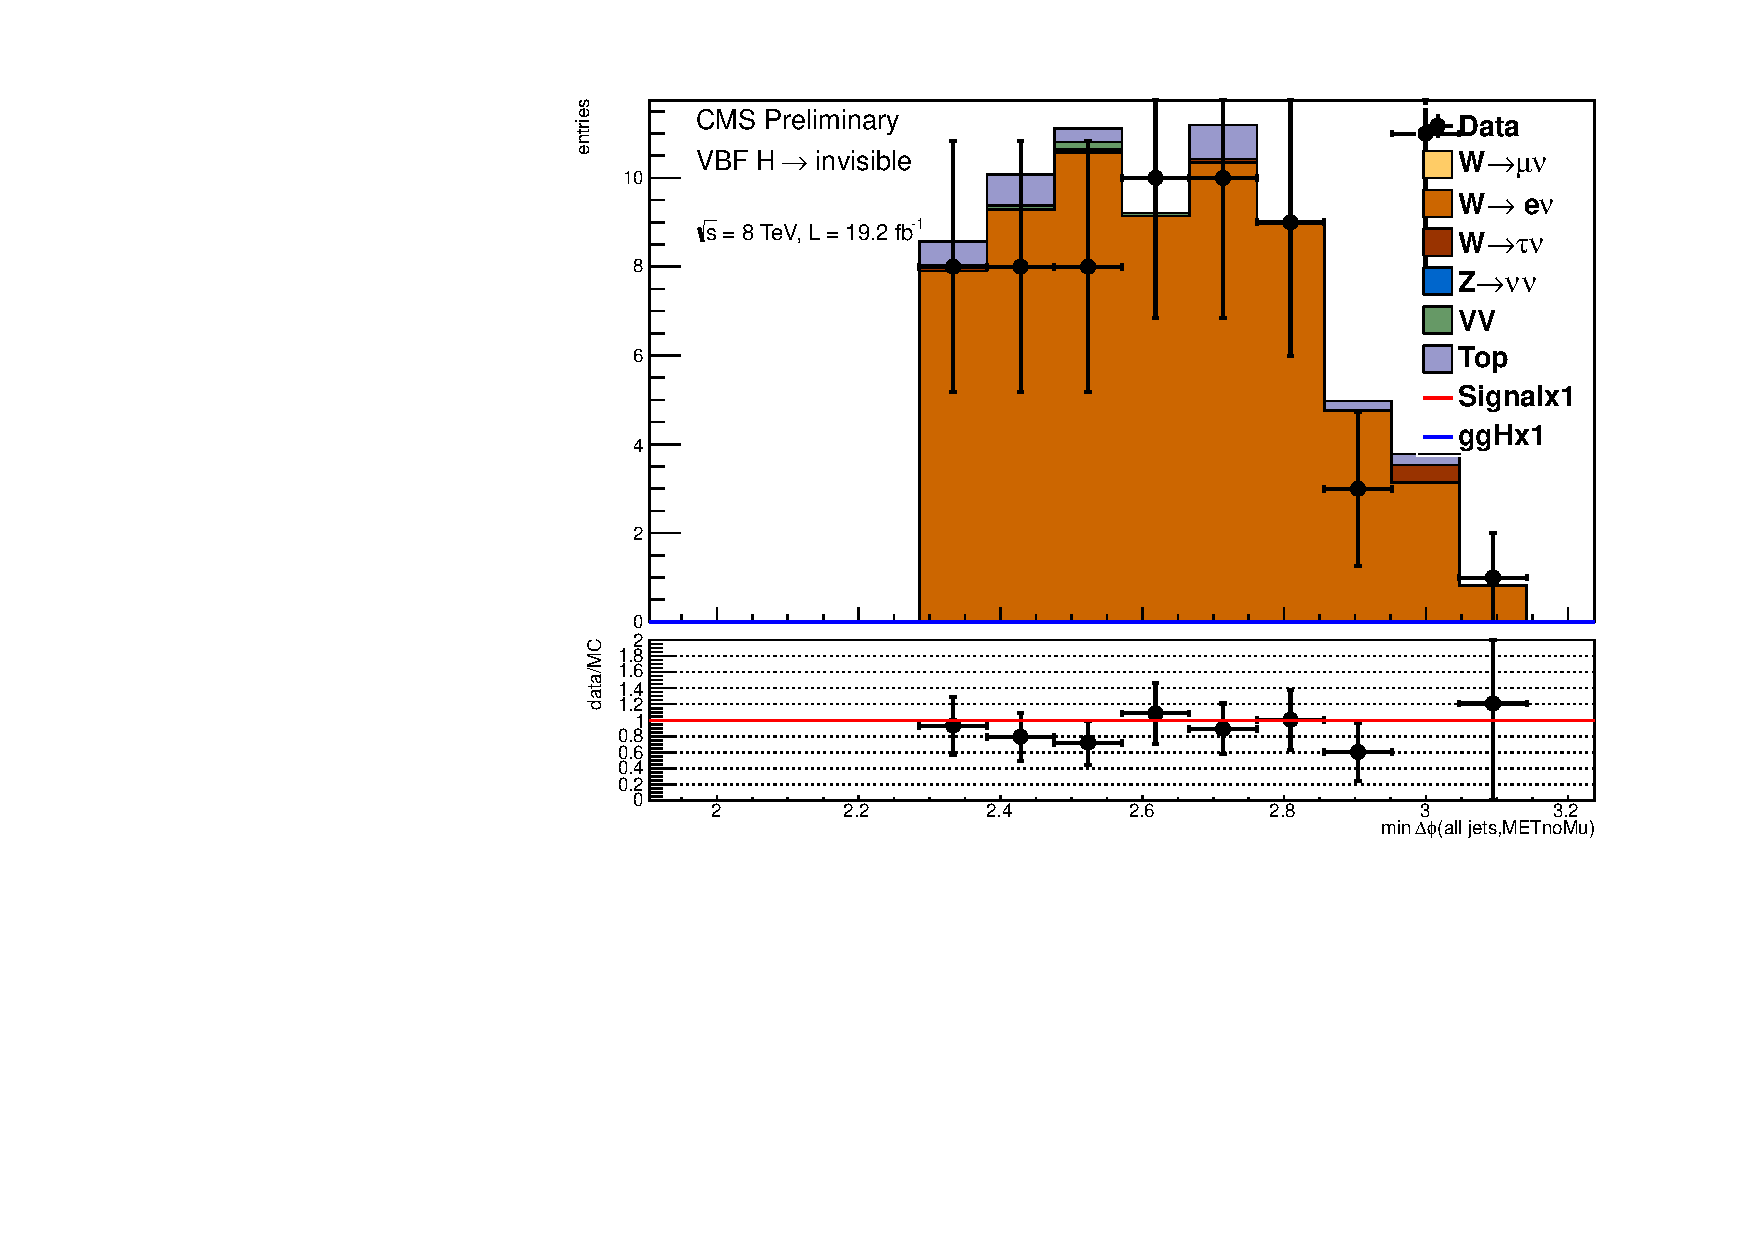
\includegraphics[width=0.49\textwidth]{figures/enu_alljetsmetnomu_mindphi.pdf}
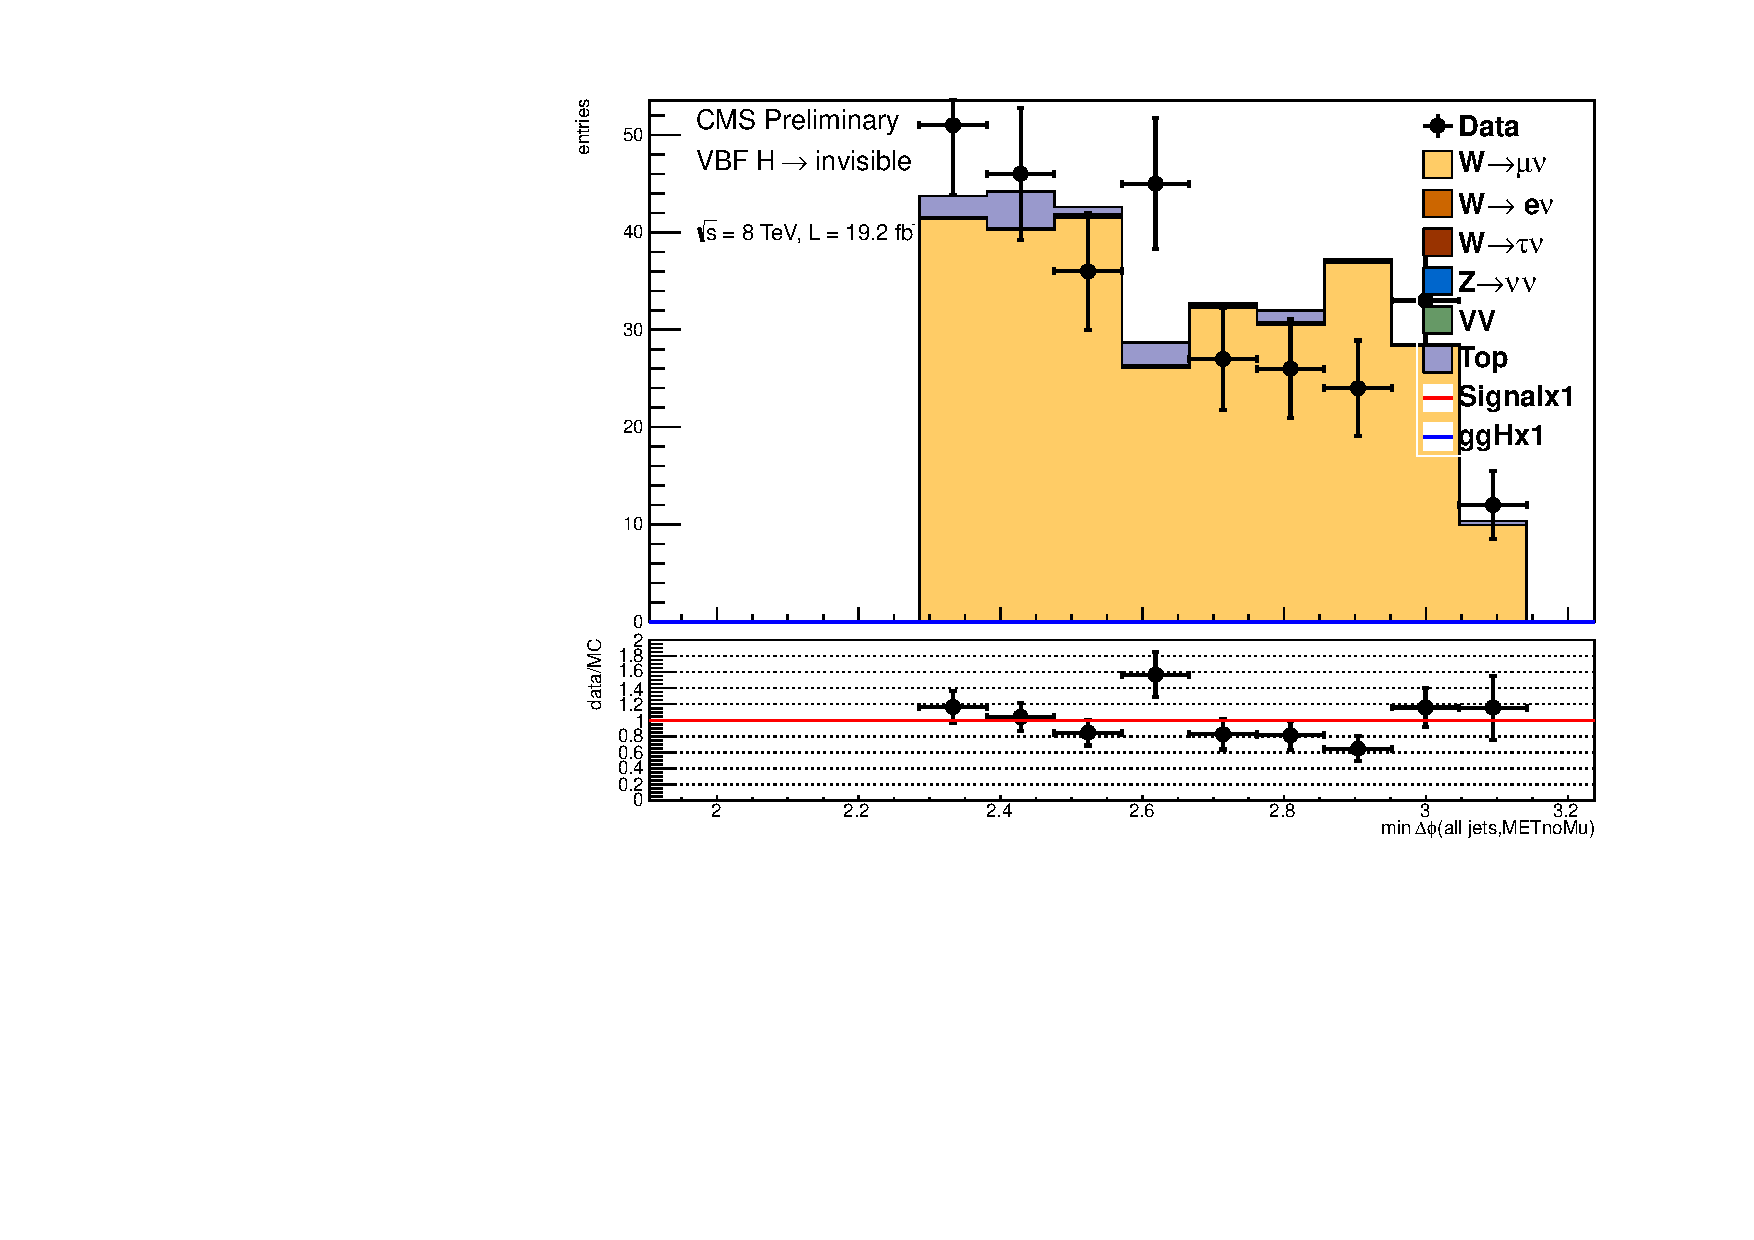
\includegraphics[width=0.49\textwidth]{figures/munu_alljetsmetnomu_mindphi.pdf}
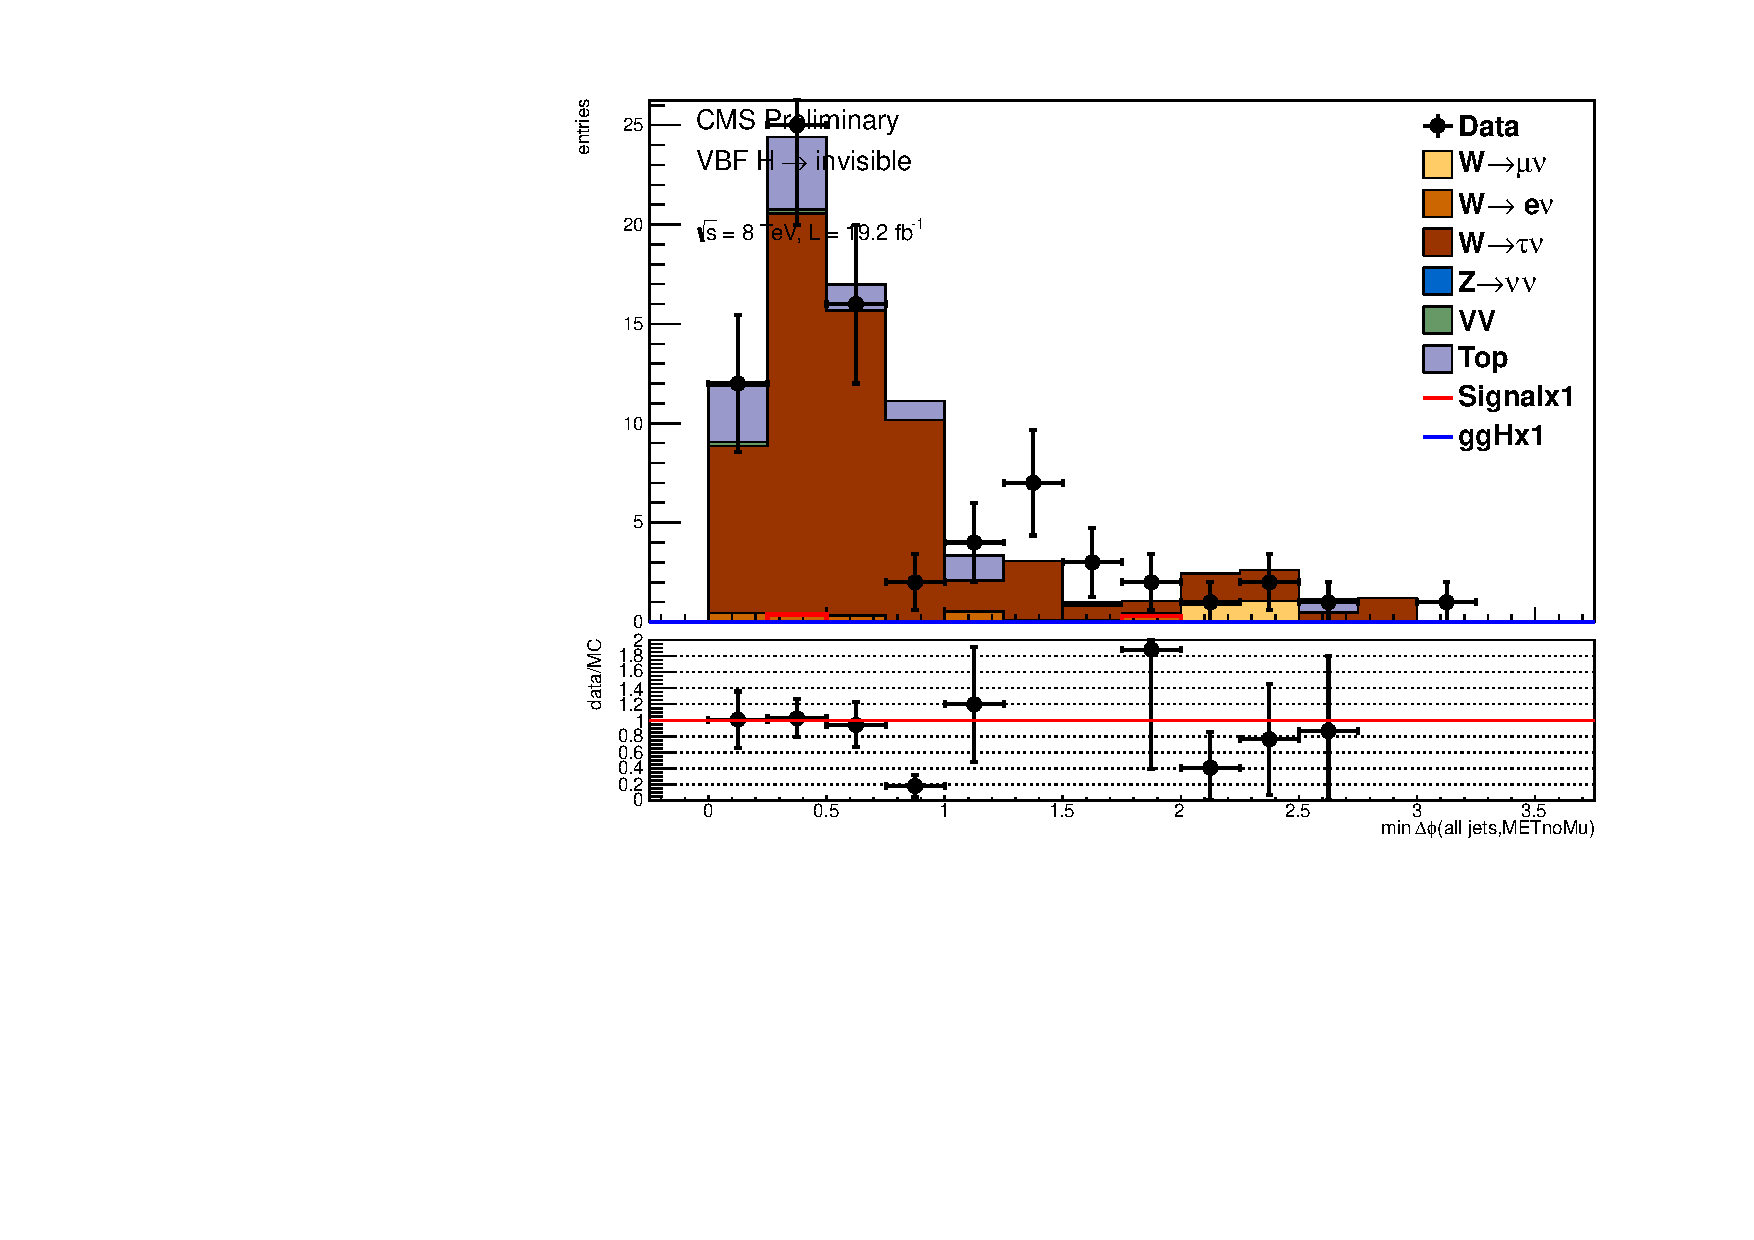
\includegraphics[width=0.49\textwidth]{figures/taunu_alljetsmetnomu_mindphi.pdf}
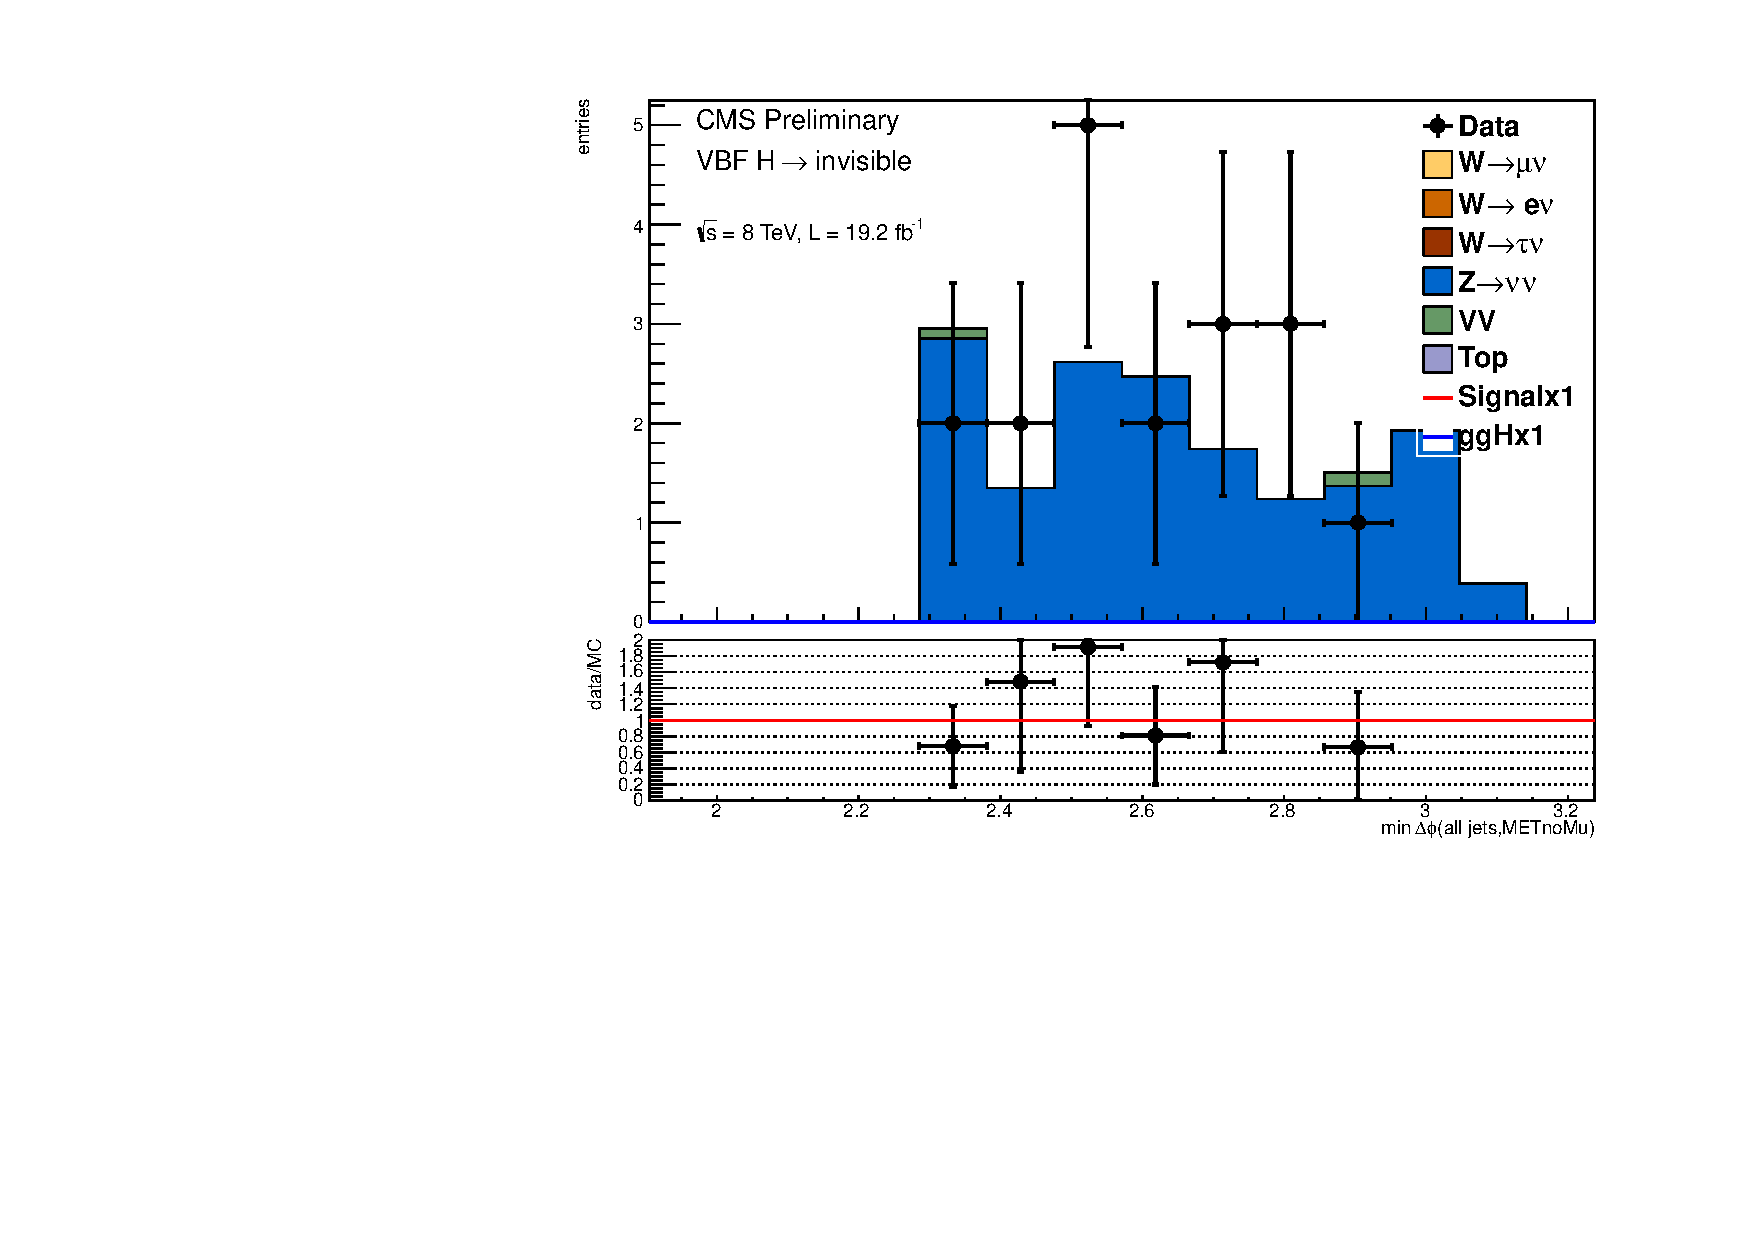
\includegraphics[width=0.49\textwidth]{figures/mumu_alljetsmetnomu_mindphi.pdf}
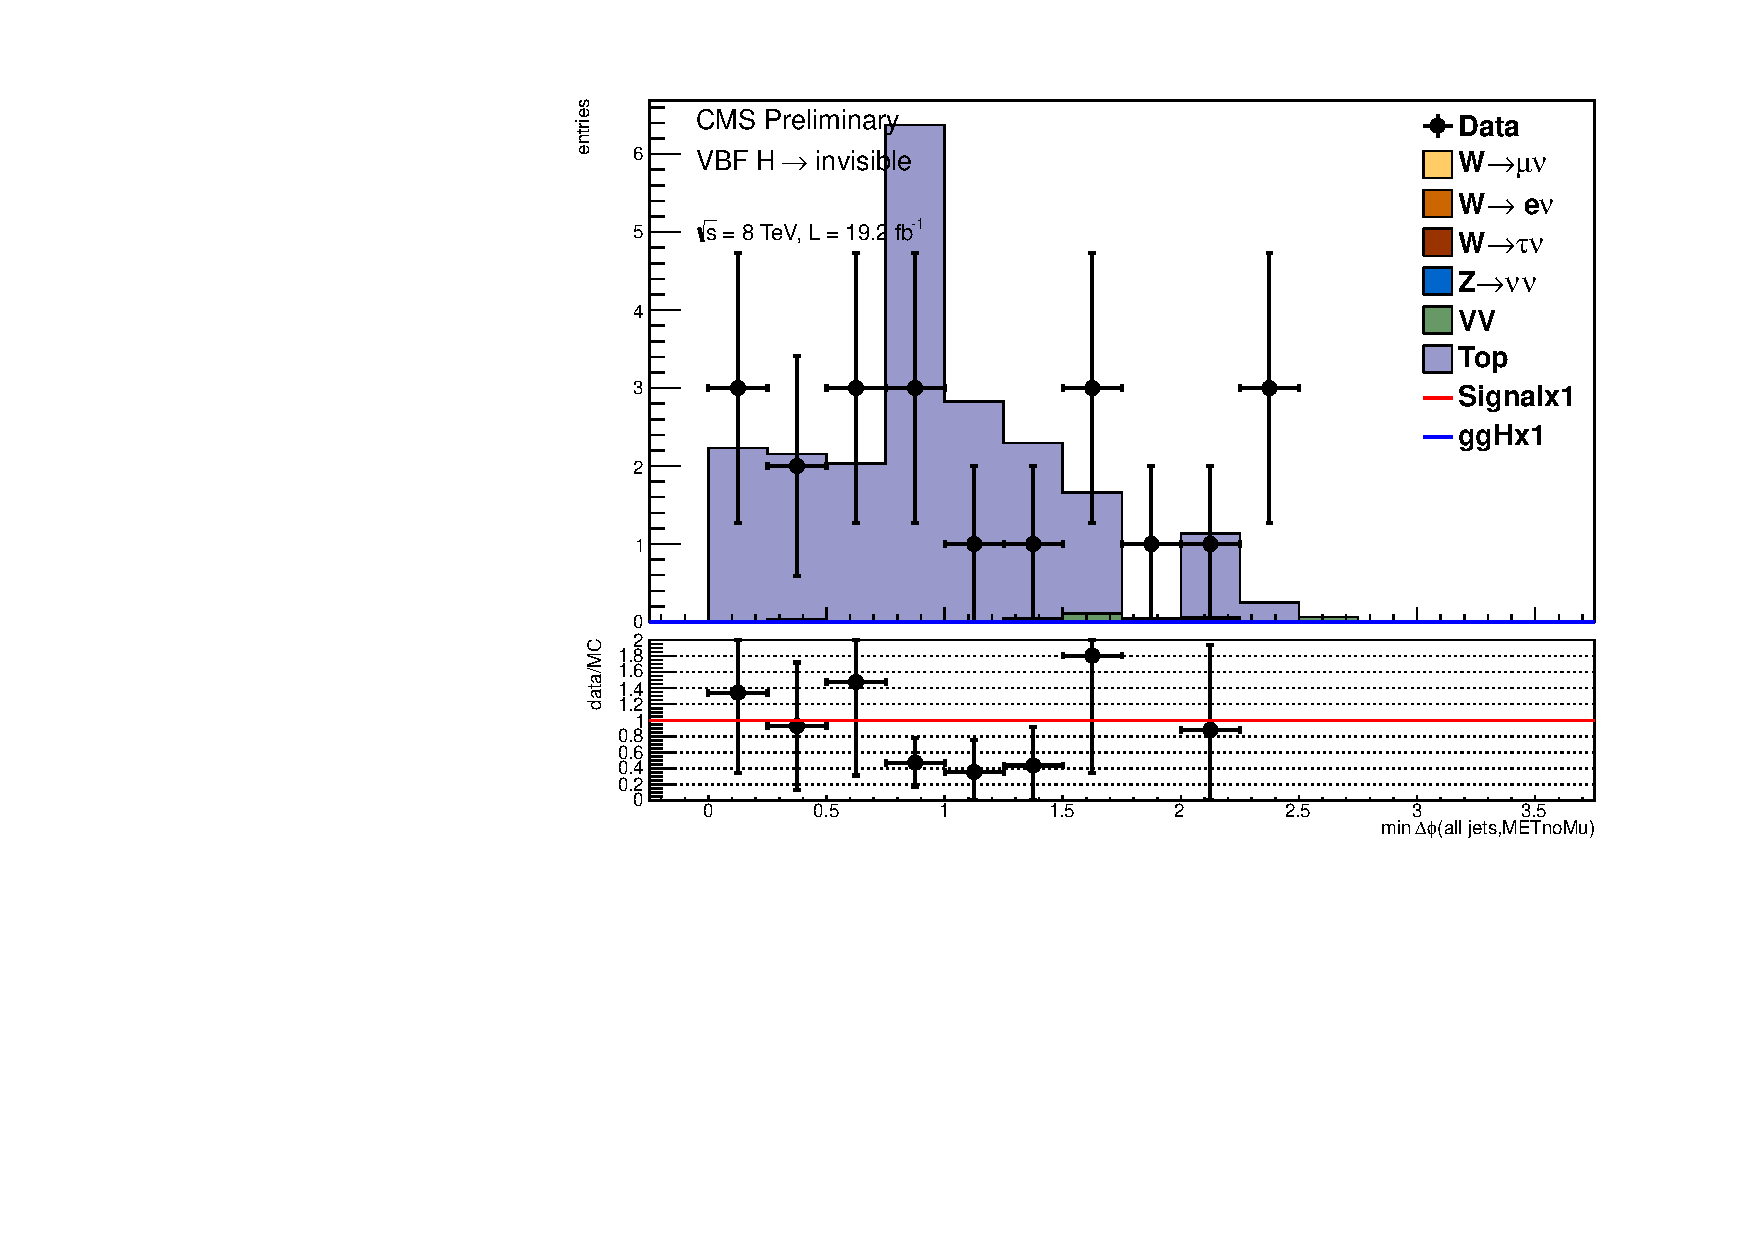
\includegraphics[width=0.49\textwidth]{figures/top_alljetsmetnomu_mindphi.pdf}
\caption{Distribution of the $\mindphiall$ variable in the data and MC, after reweighting the MC to match the data in normalisation. Top row, from left to right: W$\rightarrow e,\mu,\tau_{\mathrm{h}}$ control regions. Bottom row: left, Z$\rightarrow\mu\mu$ and top control regions.}
\label{fig:vbfCR} 
\end{center}
\end{figure*}

%!!QCD DISCRIPTION
The QCD multijet process is modelled using the sample of events where the isolation requirement on the \MET has been reversed by requiring that \mindphiall$<$1.0 but still requiring that the minimum azimuthal angle separation between the leading two jets and the \MET, \mindphileading, be greater than 2.3. We normalise these events in a sideband region to the signal region, which is dominated by QCD.
The region chosen is that with 3$<$\METsig$<$4 and 1.0$<$\mindphileading$<$2.0. It is observed that the normalisation factor has a strong dependence on \METsig and \mindphiall. To model this behaviour the normalisation factor is measured both as a function of the cut placed on \METsig and as a function of the cut placed on \mindphiall. Both functional forms are then extrapolated to the signal region cut values, and the final normalisation factor is taken to be the centre of the envelope formed by the two values obtained.

The final number of events for each process that passes the selection is estimated using
the MC in the case of the W, Z and top with jets processes, or the non-isolated \MET events for the QCD multijets process,
 with the normalisation obtained from the control regions, and is summarised in Table~\ref{tab:bgSummary}. 
The distribution of the $\mindphiall$ variable in the signal region, with all backgrounds taking their final normalisation
 is shown in Figure~\ref{fig:vbfSR}. An overview of all considered systematic uncertainties is given in
Table~\ref{tab:syst-qqH}, with the effect on the sum of all the background
processes and the signal with $\mH=125$\GeV and $\BRinv=100$\% given separately.

\begin{table*}[th!]
	\centering \caption{Summary of the estimated number of
		background and signal events, together with the
		observed yield, in the VBF search signal region.  The
		signal yield is given for $\mH=125$\GeV and
		$\BRinv=100$\%. The errors quoted are the statistical and systematic uncertainties respectively}  \label{tab:bgSummary}

\begin{tabular}{lc}   
\hline \hline                                    
Process & Event yields \\
\hline                 
$Z\rightarrow\nu\nu$&$157.3 \pm 37.6 \pm 38.3$\\
$W\rightarrow\mu\nu$&$101.8 \pm 6.1 \pm 11.9$\\
$W\rightarrow e\nu$&$57.4 \pm 7.3 \pm 7.0$\\ 
$W\rightarrow\tau\nu$&$98.0 \pm 13.2 \pm 25.4$\\
top&$4.4 \pm 1.0 \pm 1.4$\\
VV&$3.8 \pm 0.0 \pm 0.7$\\
QCD multijet &$17\pm 0 \pm14$\\
\hline
Total Background &$439.7 \pm 41.0 \pm 55.8 $\\
\hline
Signal(VBF) &$273.4 \pm 0.0 \pm 31.2 $\\
Signal(ggH) &$22.6 \pm 0.0 \pm 15.6 $\\
\hline \hline 
\end{tabular}
\end{table*}

\begin{figure*}[hbtp]
\begin{center} 
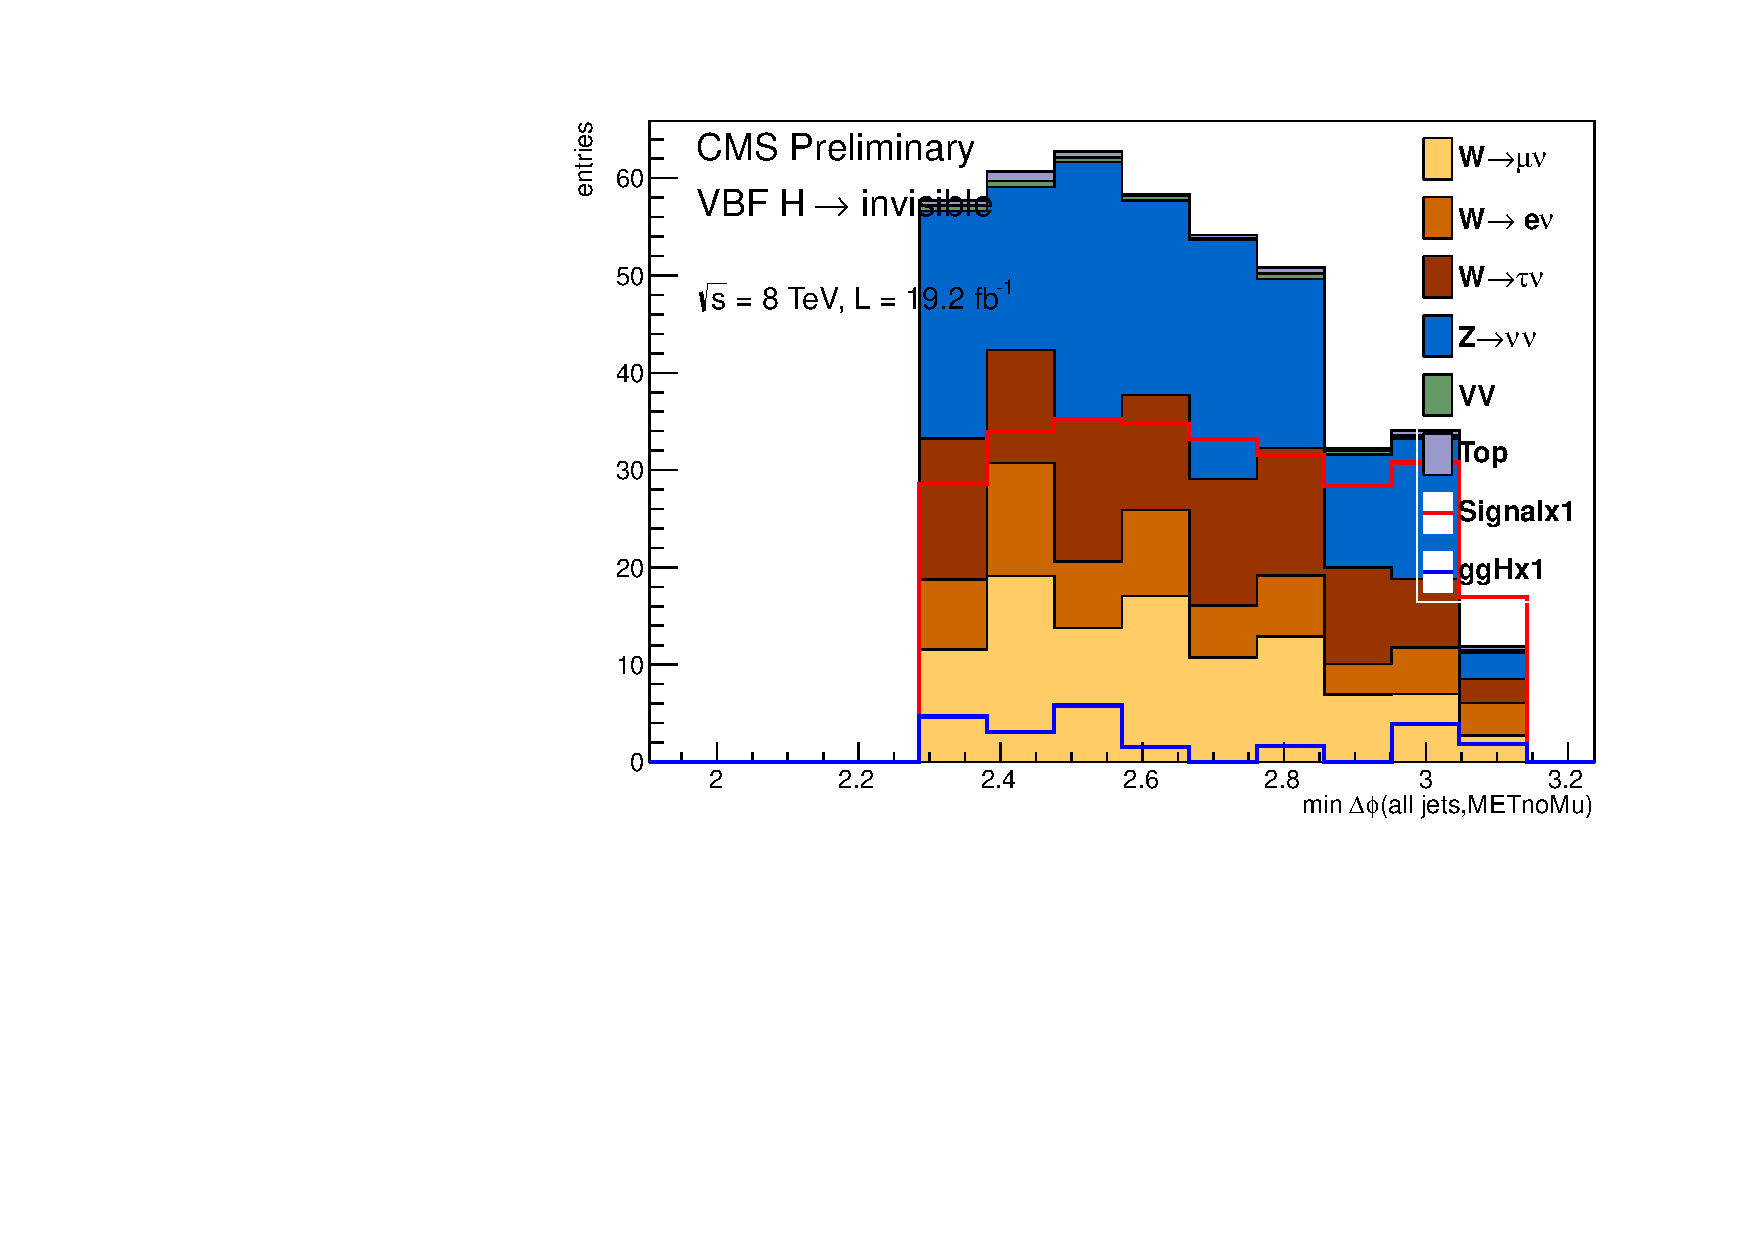
\includegraphics[width=0.49\textwidth]{figures/nunu_alljetsmetnomu_mindphi.pdf}
\caption{Distribution of the $\mindphiall$ variable in the data and MC in the signal region, with the W, Z and top backgrounds normalised to the data in their respective control regions} %!!REPLACE WITH UNBLIND VERSION WHEN WE UNBLIND
\label{fig:vbfSR} 
\end{center}
\end{figure*}

\begin{table*}[h!t]
\centering
\topcaption{Summary of the uncertainties on the total background and signal yields. All uncertainties affect the normalization of the yield, and are quoted as the change in \% in the total background or signal estimate, when each systematic effect is varied according to its uncertainties. The signal uncertainties are given for $\mH=125$\GeV and $\BRinv=100$\%.}
\label{tab:syst-qqH}
\begin{tabular}{lcc}
\hline \hline
Source	& Total background & Signal	\\
\hline
Luminosity & 0.02 & 2.60 \\ 
Electron efficiency & 0.63 & 0.00 \\ 
Muon efficiency & 2.61 & 0.00 \\ 
Jet energy scale & 4.94 & 10.70 \\ 
Jet energy resolution & 2.86 & 1.81 \\ 
Unclustered energy scale & 2.28 & 1.64 \\ 
Pileup weight & 0.95 & 1.56 \\ 
$Z\rightarrow\nu\nu$ MC stat. & 4.13 & 0.00 \\ 
$Z\rightarrow\nu\nu$ data stat. & 8.54 & 0.00 \\ 
$W\rightarrow \mu\nu$ MC stat. & 1.90 & 0.00 \\ 
$W\rightarrow \mu\nu$ data stat. & 1.40 & 0.00 \\ 
$W\rightarrow e\nu$ MC stat. & 1.34 & 0.00 \\ 
$W\rightarrow e\nu$ data stat. & 1.66 & 0.00 \\ 
Tau efficiency & 1.78 & 0.00 \\ 
$W\rightarrow\tau\nu$ control region extrapolation & 4.46 & 0.00 \\ 
$W\rightarrow\tau\nu$ MC stat. & 2.85 & 0.00 \\ 
$W\rightarrow\tau\nu$ data stat. & 3.00 & 0.00 \\ 
$Z/\gamma^{*}\rightarrow\mu\mu$ to $Z\rightarrow\nu\nu$ extrapolation & 7.16 & 0.00 \\ 
Top MC stat. & 0.30 & 0.00 \\ 
Top data stat. & 0.22 & 0.00 \\ 
QCD normalisation & 0.00 & 0.00 \\ 
VV MC stat. & 0.11 & 0.00 \\ 
VV cross-section & 0.01 & 0.00 \\ 
VBF MC stat. & 0.00 & 3.13 \\ 
VBF QCD scale & 0.00 & 0.18 \\ 
VBF pdf & 0.00 & 2.49 \\ 
ggH MC stat. & 0.00 & 2.19 \\ 
ggH QCD scale & 0.00 & 4.22 \\ 
ggH pdf & 0.00 & 0.86 \\ 
UEPS & 0.00 & 1.28 \\
\hline \hline
\end{tabular}
\end{table*}

The dominant uncertainties come from the statistical
uncertainty on the number of data events in each of the control
regions. In order to estimate the effect of the jet energy scale,
unclustered energy scale and jet energy resolution on both the signal
and background processes, each quantity is varied separately by its
uncertainties in both directions and the full background and signal estimation are
repeated. Similarly, the pileup and lepton efficiency scale factors
applied to the MC are varied by their uncertainties in both
directions. The luminosity uncertainty of 2.6\% and the trigger
efficiency uncertainty are applied only to the signal and to the minor
backgrounds estimated purely from MC. The data-driven normalisation
for the main backgrounds ensures that the trigger plateau is properly
taken into account. The uncertainties on the diboson cross sections
are taken from the CMS published cross-section
measurements~\cite{Chatrchyan:2013oev}.

Further uncertainties come from the theoretical uncertainty on the
cross-section ratio used to extrapolate from QCD produced
$Z/\gamma^{*}\rightarrow\mu\mu$ to $Z\rightarrow\nu\nu$ in the
$Z\rightarrow\nu\nu$ background estimation. This uncertainty is
estimated by calculating the ratio of yields obtained from both MCFM
and MadGraph in a VBF dominated region for both processes. The MCFM
NLO result is found to be 1.14, while MadGraph gives $1.2\pm0.2$
resulting in a 20\% uncertainty on the $Z\rightarrow\nu\nu$ estimate
to account for this difference. Theoretical uncertainties on the
signal cross-sections due to PDF and QCD scales are taken from the LHC
Higgs Cross Section Working Groups Yellow Report
3~\cite{Dittmaier:2011ti,Dittmaier:2012vm}.

Upper limits on the Higgs boson production cross section times \BRinv
are placed at 95\% C.L. using an
asymptotic CLs method\cite{Read1,junkcls,LHC-HCG}, following the
standard CMS Higgs combination technique~\cite{Chatrchyan:2013lba,HiggsCombination}.
Systematics uncertainties are treated as nuisance parameters in a frequentist paradigm as described in Ref.~\cite{HiggsCombination},
and all correlations between processes are taken into account.

Using this procedure and assuming SM Higgs boson production cross-sections and acceptances,
 the observed (median expected) 95\% C.L. limit on \BRinv
 of a SM 125 GeV Higgs boson is XX (38)\%. The 95\% C.L. limit on %!!ADD OBSERVED WHEN WE UNBLIND
\BRinv and the 95\% C.L. limit on the cross-section times \BRinv, both assuming SM Higgs boson acceptances are
shown as a function of Higgs boson mass in figure \ref{fig:limits}.

\begin{figure}[h!]
  \begin{center}
    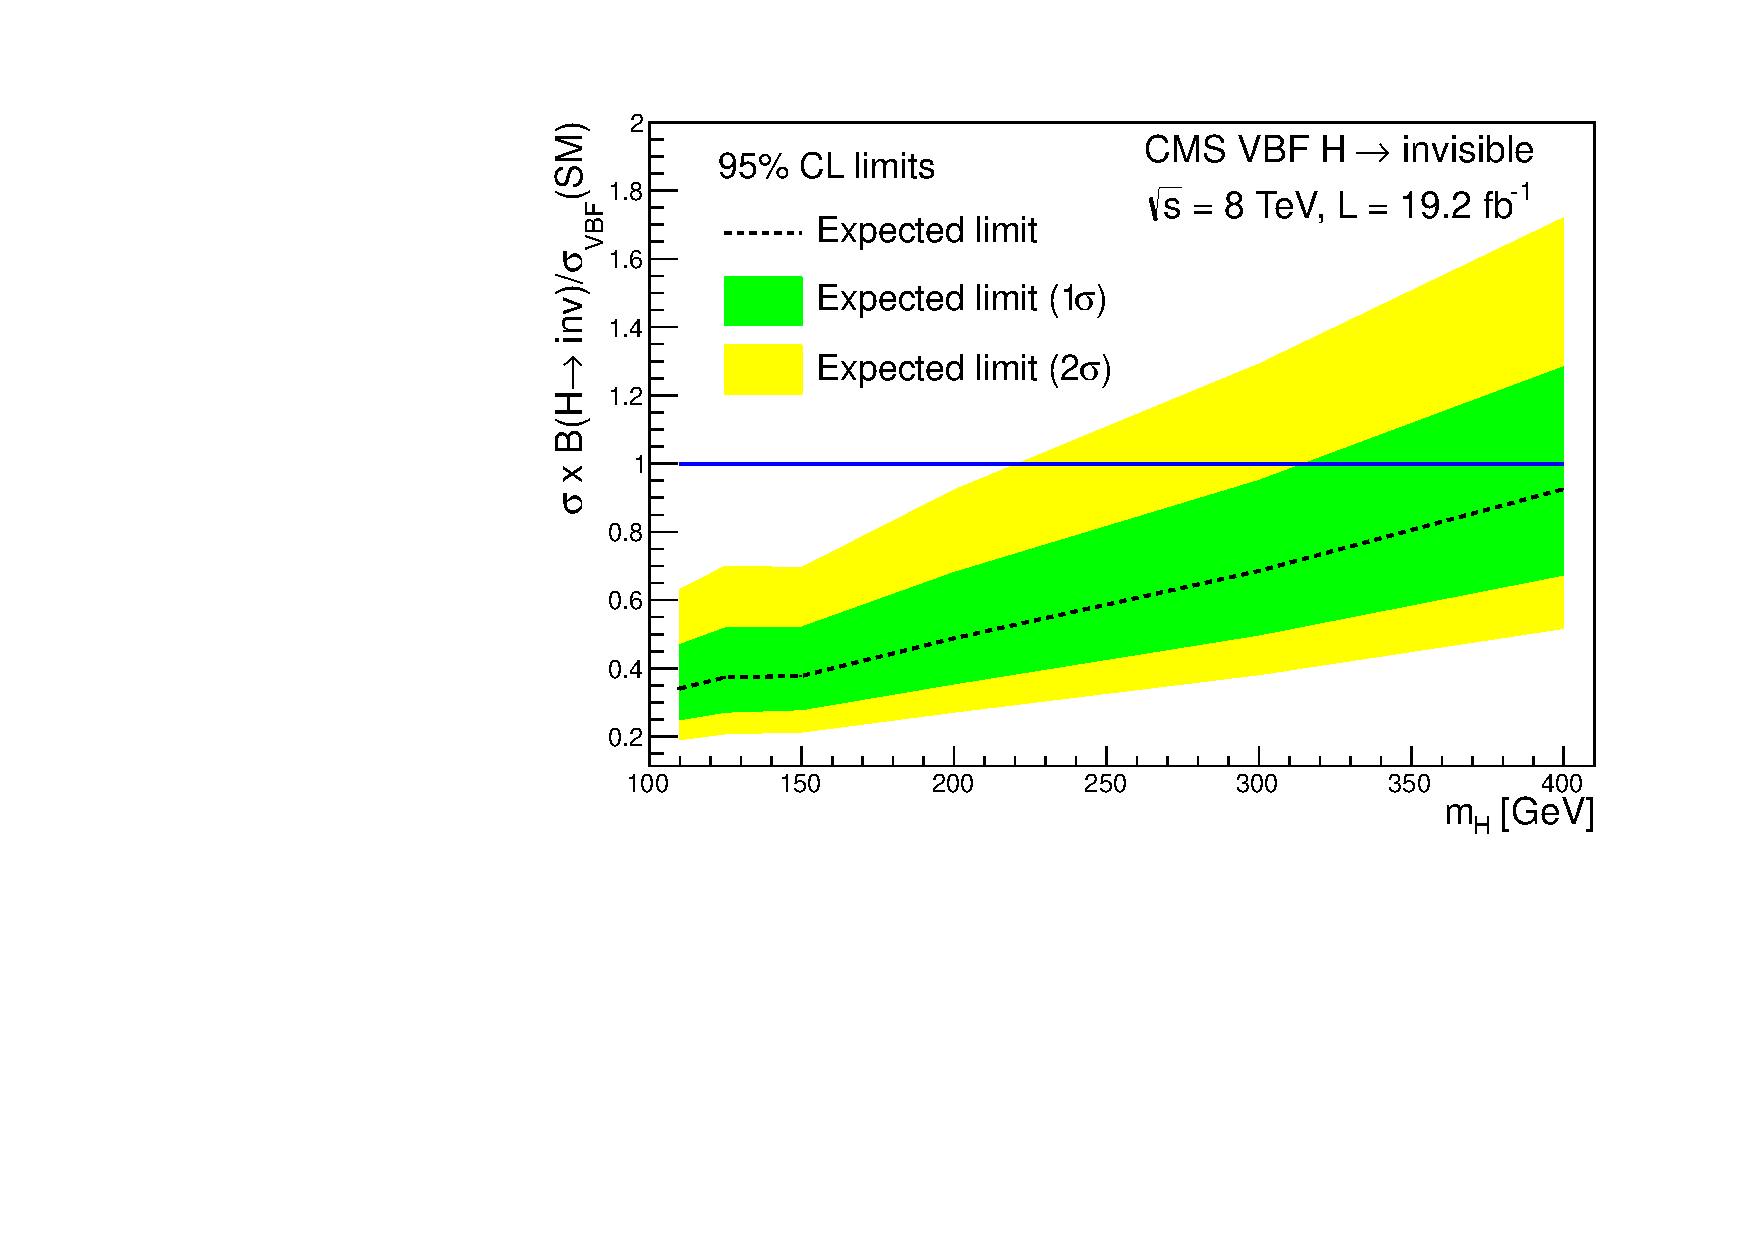
\includegraphics[width=0.49\textwidth]{figures/vbflimit.pdf}
    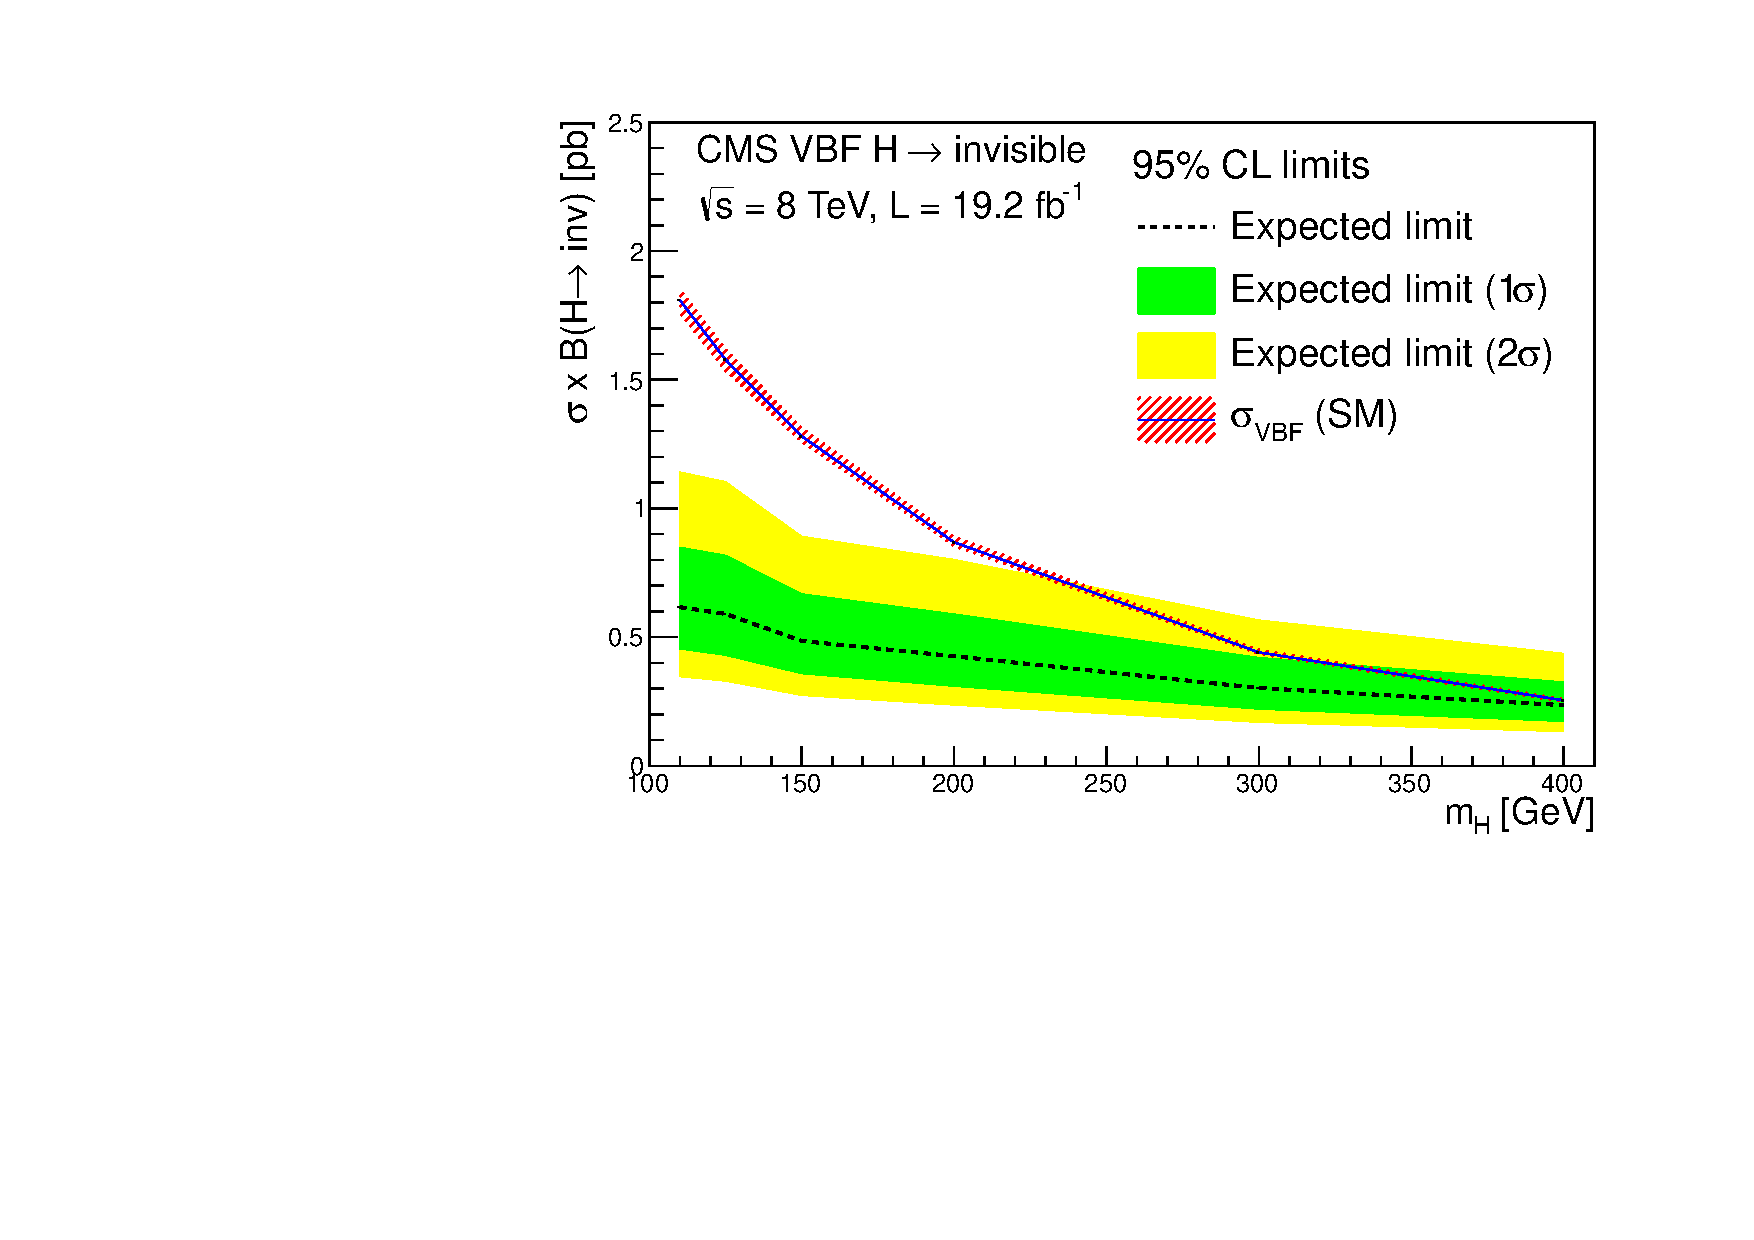
\includegraphics[width=0.49\textwidth]{figures/vbfxslimit.pdf}
 \caption{The 95\% C.L. limit on \BRinv of a SM Higgs
boson (\cmsLeft) and the 95\% C.L. limit on the cross-section times
\BRinv (\cmsRight)as a function of the Higgs
boson mass, assuming SM Higgs boson acceptances.}
    \label{fig:limits}
  \end{center}
\end{figure}




%conclusion
A search for VBF produced Higgs bosons decaying to invisible final states has been performed.
The analysis' sensitivity is increased significantly by the use of triggers 
recorded as part of the parked data stream. These triggers allow the use a selection driven by enhancing the
contribution from \MET coming from genuine invisible particles isolated from jet activity in the transverse plane,
 rather than mismeasured energy or \MET from heavy-flavoured jet decays. 
The observed (median expected) limit on \BRinv
 of a SM Higgs with $\mH=125$\GeV is XX (38)\%, which is an improvement in sensitivity of 
more than 20\% compared to the previous CMS analysis.



% >> acknowledgements (for journal papers)
% Please include the latest version from https://twiki.cern.ch/twiki/bin/viewauth/CMS/Internal/PubAcknow.
\section*{Acknowledgements}
{\tolerance=900 

We congratulate our colleagues in the CERN accelerator departments for the excellent performance of the LHC and thank the technical and administrative staffs at CERN and at other CMS institutes for their contributions to the success of the CMS effort. In addition, we gratefully acknowledge the computing centres and personnel of the Worldwide LHC Computing Grid for delivering so effectively the computing infrastructure essential to our analyses. Finally, we acknowledge the enduring support for the construction and operation of the LHC and the CMS detector provided by the following funding agencies: BMWFW and FWF (Austria); FNRS and FWO (Belgium); CNPq, CAPES, FAPERJ, and FAPESP (Brazil); MES (Bulgaria); CERN; CAS, MoST, and NSFC (China); COLCIENCIAS (Colombia); MSES and CSF (Croatia); RPF (Cyprus); MoER, ERC IUT and ERDF (Estonia); Academy of Finland, MEC, and HIP (Finland); CEA and CNRS/IN2P3 (France); BMBF, DFG, and HGF (Germany); GSRT (Greece); OTKA and NIH (Hungary); DAE and DST (India); IPM (Iran); SFI (Ireland); INFN (Italy); MSIP and NRF (Republic of Korea); LAS (Lithuania); MOE and UM (Malaysia); CINVESTAV, CONACYT, SEP, and UASLP-FAI (Mexico); MBIE (New Zealand); PAEC (Pakistan); MSHE and NSC (Poland); FCT (Portugal); JINR (Dubna); MON, RosAtom, RAS and RFBR (Russia); MESTD (Serbia); SEIDI and CPAN (Spain); Swiss Funding Agencies (Switzerland); MST (Taipei); ThEPCenter, IPST, STAR and NSTDA (Thailand); TUBITAK and TAEK (Turkey); NASU and SFFR (Ukraine); STFC (United Kingdom); DOE and NSF (USA).

\par}
%% **DO NOT REMOVE BIBLIOGRAPHY**
\bibliography{auto_generated}   % will be created by the tdr script.

%% examples of appendices. **DO NOT PUT \end{document} at the end
%\clearpage
%\appendix
%\section{PTDR Symbol Definitions\label{app:symdef}}

%%% DO NOT ADD \end{document}!

